\section{Extensive game}

\begin{definition}[\textit{Extensive form game with perfect information}]
    An extensive form game with perfect information consists of: 
    \begin{enumerate}
        \item A finite set $N = \{1,\dots,n\}$ of players. 
        \item A game tree $(V,E,x_0)$.
        \item A partition of the vertices that are not leaves into sets ${P1, P2, \dots , Pn+1}$.
        \item A probability distribution for each vertex in $P_{n+1}$, defined on the edges from the vertex to its children.   
    \end{enumerate}
\end{definition}
We have the following: 
\begin{enumerate}
    \item The set $P_i$ , for $i \leq n$, is the set of the nodes $v$ where Player $i$ must choose a child of $v$, representing a possible move from him at $v$.
    \item $P_{n+1}$ is the set of the nodes where a chance move is present: that is $n + 1$ is the number of players plus the random component. 
        $P_{n+1}$ can be empty, meaning that the game does not admit any chance.
    \item When $P_{n+1}$ is empty, the $n$ players have only preferences on the leaves: a utility function is not required. 
\end{enumerate}

\subsection{Solving an extensive game}
In order to find the optimal outcome, we employ the rationality axioms. 
\begin{example}
    For the voting game described before: 
    \begin{figure}[H]
        \centering
        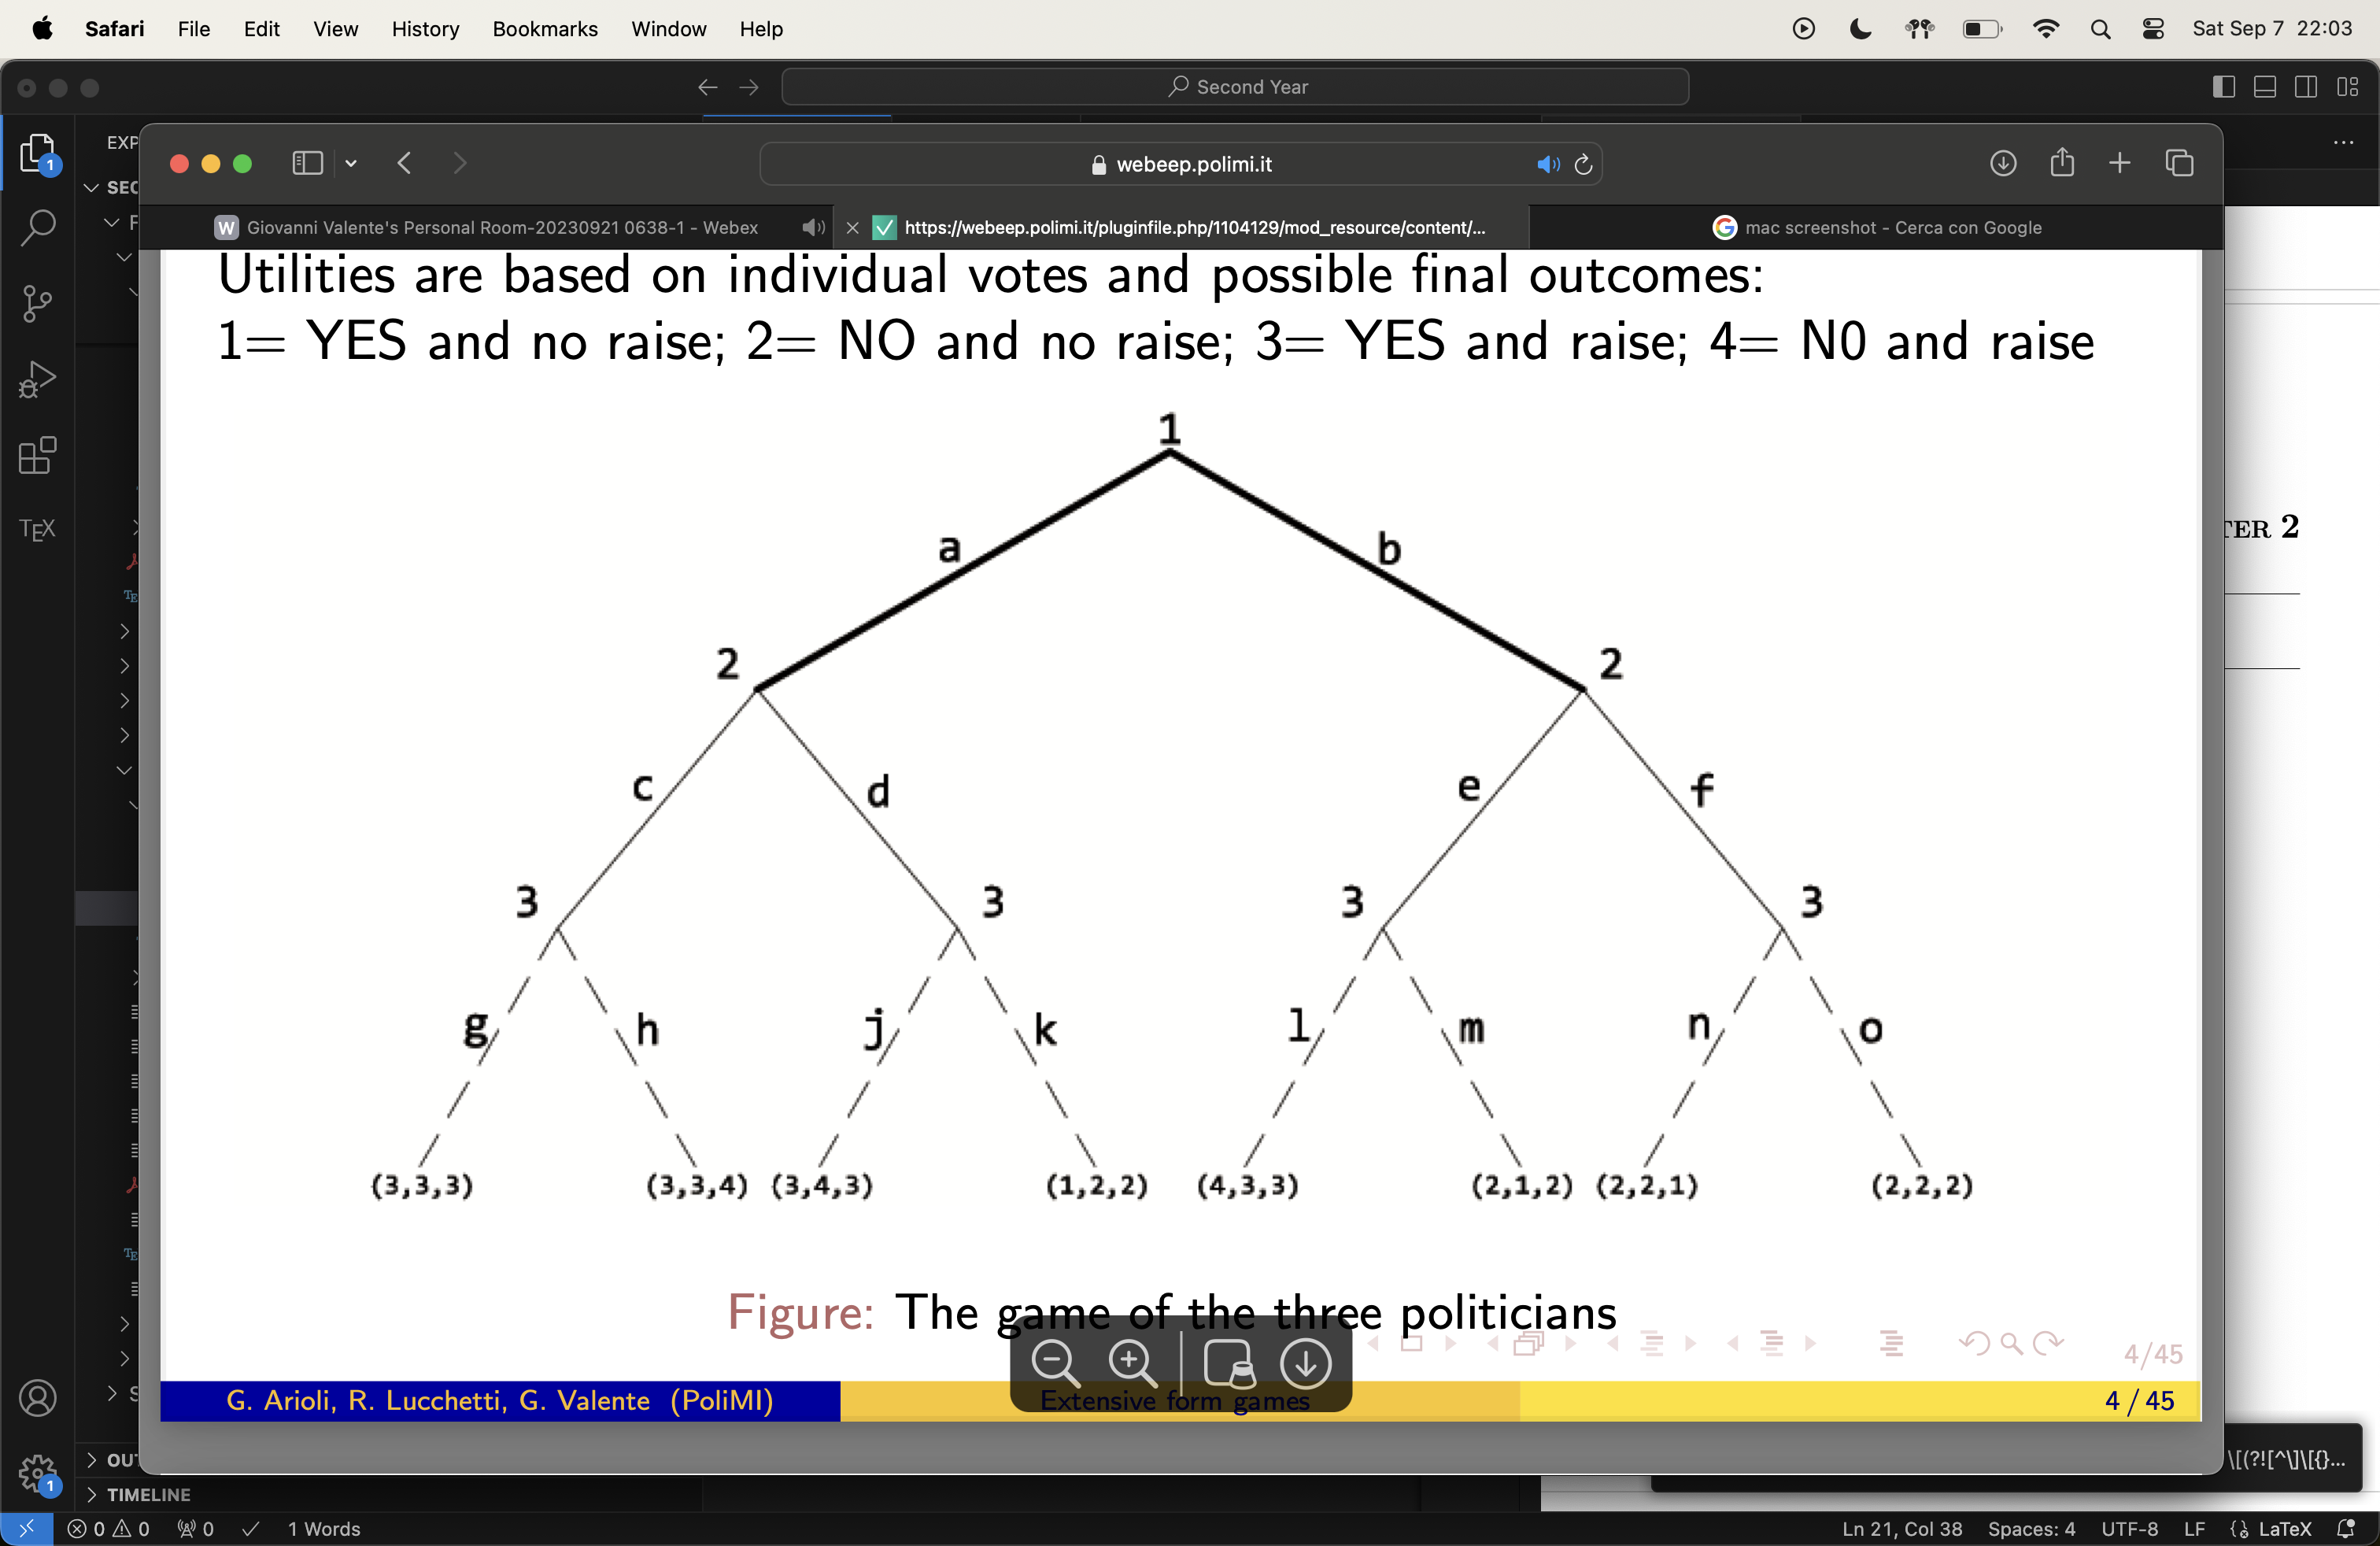
\includegraphics[width=0.75\linewidth]{images/tree.png}
        \caption{Voting game tree}
    \end{figure}
    We have the following: 
    \begin{itemize}
        \item Player3: h = (3, 3, 4) over g = (3, 3, 3) ; j = (3, 4, 3) over k = (1, 2, 2); l = (4, 3, 3) over m= (2, 1, 2) ; o = (2, 2, 2) over n= (2, 2, 1)
        \item Player2: d =(3,4,3)overc =(3,3,4);e =(4,3,3)overf =(2,2,2) 
        \item Player1: b = (4, 3, 3) over a = (3, 4, 3), thereby finding the optimal outcome
    \end{itemize}
\end{example}
\begin{definition}[\textit{Length}]
    Define Length of the game as the length of the longest path in the game.
\end{definition}
Decision theory, i.e. rationality assumption 5, enables us to solve games of length $1$. 
Rationality assumption 4 allows us to solve a game of length $i + 1 $if the games of length at most $i$ are solved.
Thus, by repeated applications, we can solve games of any finite length.
This method takes the name of backward induction: it is the process of reasoning backwards in time (that is from the leaves of the tree up to the root), so as to determine a sequence of actions leading one to the optimal outcome.

\begin{theorem}[First rationality theorem]
    The rational outcomes of a finite, perfect information game are those given by the procedure of backward induction.
\end{theorem}
The method of backwards induction can be applied since every vertex $v$ of the game is the root of a new game, made by all followers of v in the initial game.
Such a game is called a subgame of the original one.
\begin{example}
    For the second game: 
    \begin{figure}[H]
        \centering
        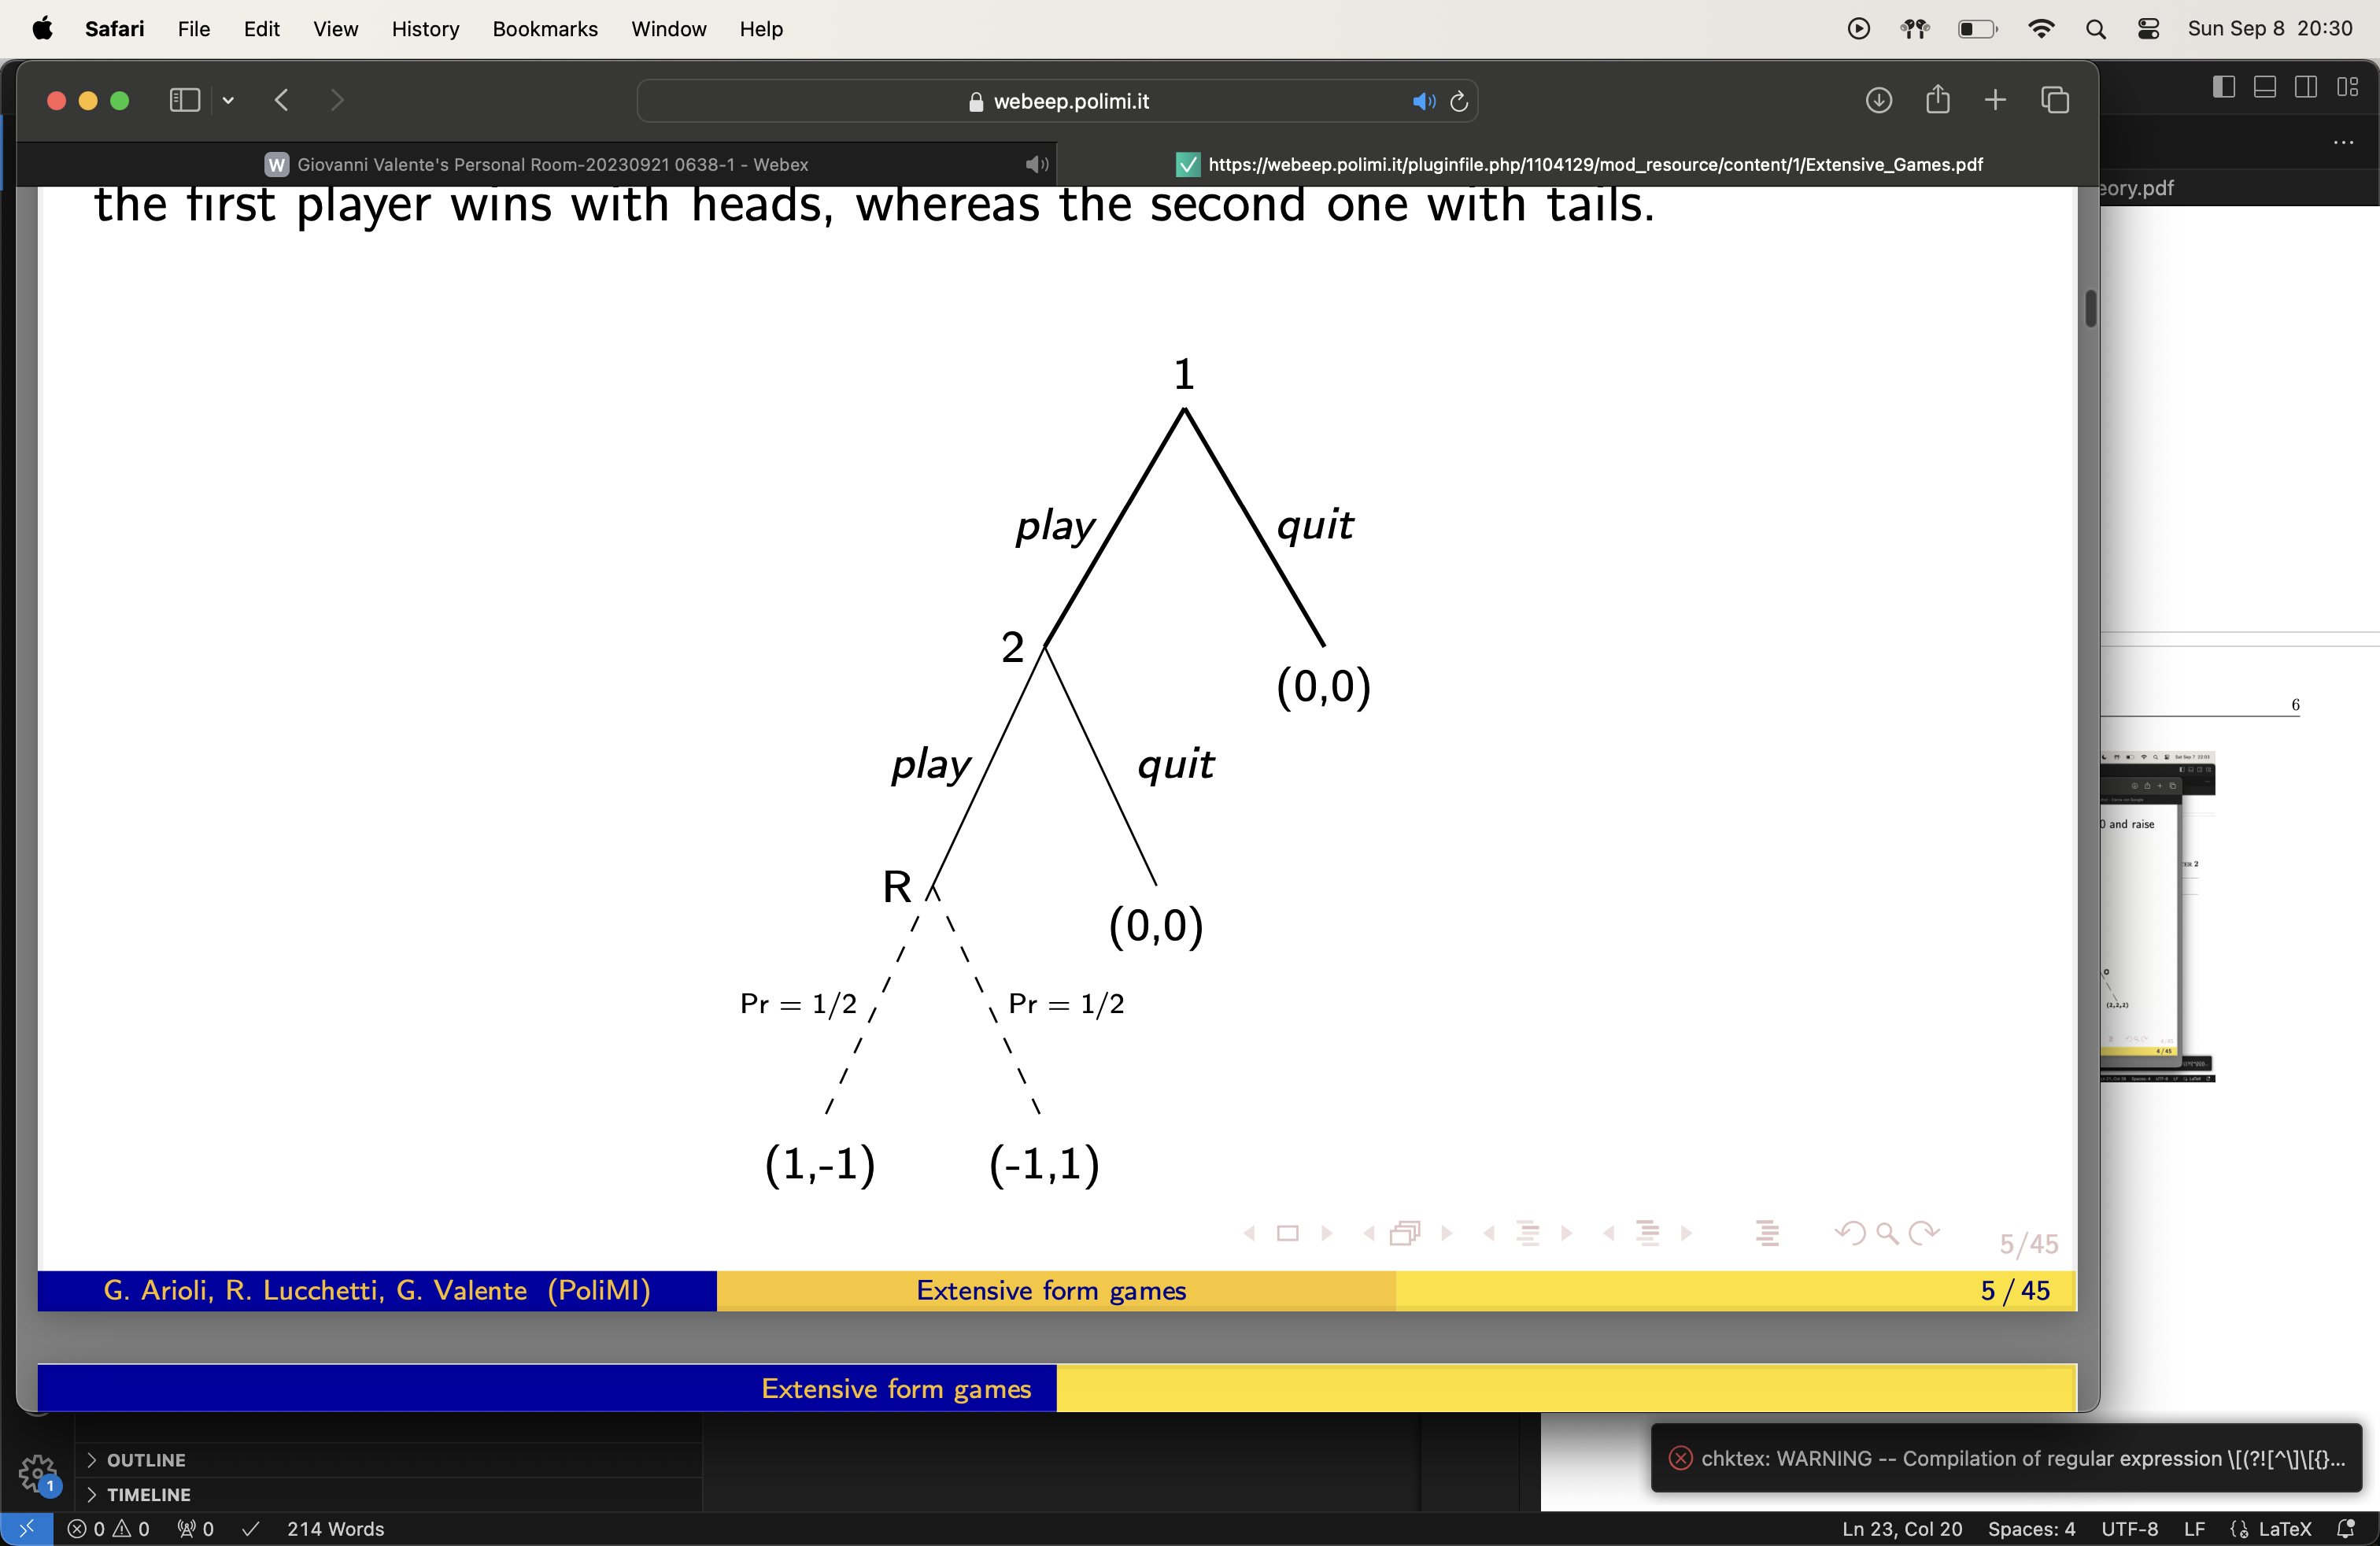
\includegraphics[width=0.75\linewidth]{images/tree1.png}
        \caption{Chance game tree}
    \end{figure}
    The outcomes obtained by backward induction are: (4, 3) and (3, 4). In fact, Pl2 does not have any preference between (4, 3) and (0, 3)!
    Therefore, in general, uniqueness of solutions is not guaranteed. 
\end{example}